\documentclass[12pt,a4paper,twoside,openright,titlepage]{article}
\usepackage[left=2cm,right=2cm,top=2cm,bottom=2cm]{geometry}

\usepackage{graphicx}
\usepackage{hyperref}
\usepackage{gensymb}
\usepackage{listings}
\usepackage{xcolor}
\usepackage{imakeidx}
\makeindex[intoc]

\definecolor{codegreen}{rgb}{0,0.6,0}
\definecolor{codegray}{rgb}{0.5,0.5,0.5}
\definecolor{codepurple}{rgb}{0.58,0,0.82}
\definecolor{backcolour}{rgb}{0.95,0.95,0.92}

\lstdefinestyle{mystyle}{
    backgroundcolor=\color{backcolour},   
    commentstyle=\color{codegreen},
    keywordstyle=\color{magenta},
    numberstyle=\tiny\color{codegray},
    stringstyle=\color{codepurple},
    basicstyle=\ttfamily\footnotesize,
    breakatwhitespace=false,         
    breaklines=true,                 
    captionpos=b,                    
    keepspaces=true,                 
    numbers=left,                    
    numbersep=5pt,                  
    showspaces=false,                
    showstringspaces=false,
    showtabs=false,                  
    tabsize=2
}
 
\lstset{style=mystyle}


\author{Bradley van Ree}
\title{FlyingKoala Introduction}

\begin{document}

\begin{titlepage}
   \begin{center}
       \vspace*{1cm}
 
       \textbf{FlyingKoala}
 
       \vspace{2cm}
 
       \textbf{Bradley van Ree}
 
       \vspace{2cm}
 
       Defining mathematical and technical models in MS Excel with Excel formulae but evaluating them using Python
 
\vfill 
 
		\begin{figure*}[h!]
			\centering
			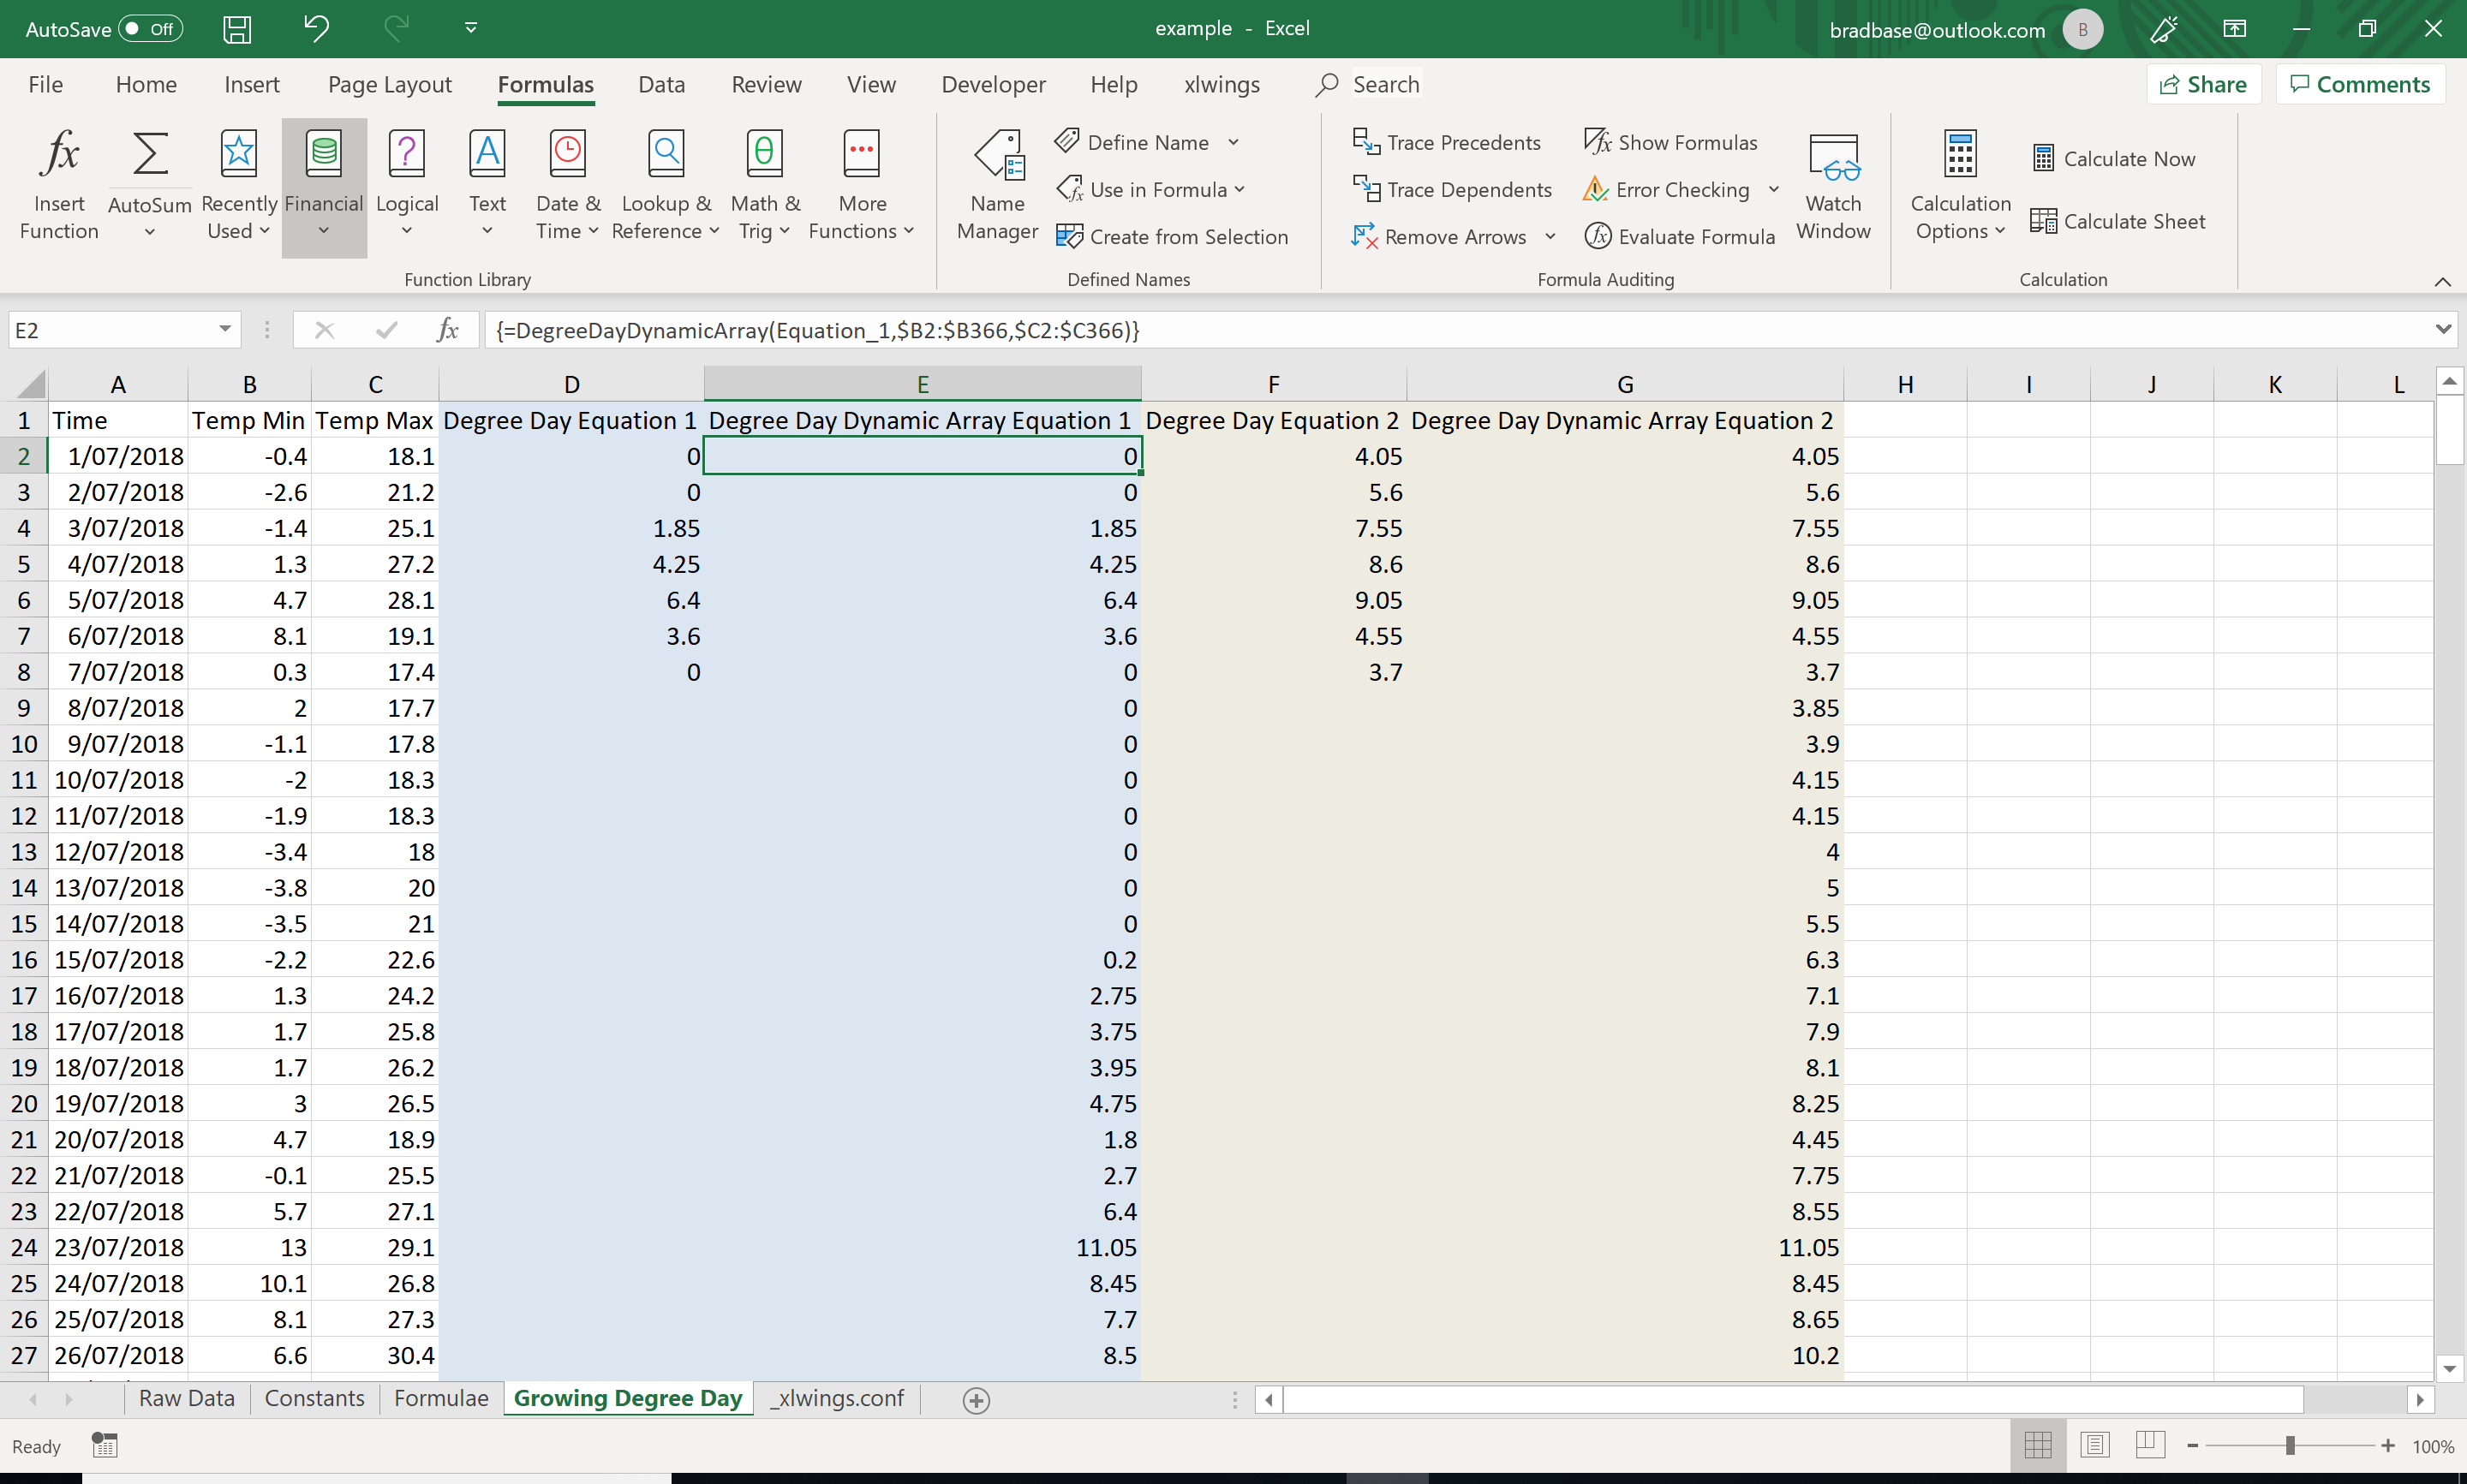
\includegraphics[scale=0.4]{images/degreedaydynamicarray_equation_1.PNG}
		\end{figure*}
 
\vfill 
 
       For use with mathematical modelling where you want the advantages of Python calculation and/or libraries but your user base are non-technical
       
       \vfill
 
   \end{center}
\end{titlepage}

\tableofcontents

\newpage 

\section{TL;DR}
\paragraph{} Srsly, I need my life back. Get to the point.

\subsection{The problem}
\begin{itemize}
	\item Data analysis with interesting data sets (large or time series) is hard
	\item Excel can get in the way just as your data set becomes interesting
	\item Not everyone is going to learn to code, nor should they be expected to
	\item Domain experts and students are usually skilled enough in MS Excel
	\item Managers can't read code to see if a mathematical (/technical) model has been created correctly
	\item Auditing is difficult when everything is in code (They don't call it code for nothing!!)
	\item Scenario analysis usually requires a heap of overhead and is difficult to manage

\end{itemize}

\subsection{Features}
\begin{itemize}
	\item MS Excel as a user interface to Python, notably Pandas (Dataframes), numpy, matplotlib, database connectivity, APIs like Harvest (timesheeting), Xero (accounting), etc\ldots
	\item matplotlib graphs in Excel
	\item xlwings has a groovy SQL feature which does magical things
	\item Excel equations are defined in Excel but processed in Python with minimal code
	\item Results of Python calculations are available in Excel
\end{itemize}


\subsection{Benefits}
\begin{itemize}
	\item The entire mathematical (/technical) model is available for managers to read because it's an Excel equation. 
	\item Audits are easier because people know how to read and change Excel
	\item inter-company expressions of a calculation don't necessarily require all sides to have evenly skilled coders
	\item Makes time series data calculations with serious size data sets possible in Excel
	\item Makes big data calculations in Excel quicker
	\item Restricts the need for a coder geek from being involved in the model development process reducing time and errors
	\item Multiple mathematical models can be defined and assessed quickly. Great for scenario analysis.
\end{itemize}

\newpage
\section{Why FlyingKoala?}

\paragraph{} While doing data analysis work, particularly time series analysis (but not necessarily limited to), you very quickly find that the limits of Excel are much closer than you'd like.

\paragraph{} The data analysis world has looked around for solutions and adapted the statistics powerhouse language R to Python forming the basis for the Pandas library. Due to the power of the Python community, matplotlib is often associated for the inevitable visualisations. And they are marvellous tools but are not necessarily intuitive. 

\paragraph{} There comes a challenge, however, when you have a number of experts who aren't necessarily code savvy but are still required to do some number crunching. These people could be engineers, finance (accountants, book keepers), sales people, specialists in quite unrelated fields like biology, botany, research or even students in essentially any field. Often enough these people are adept at Excel but are, understandably, not going to become proficient in writing computer code.

\paragraph{} It would be great if there were a solution which could take advantage of the abundantly available Excel skills and minimise the amount of computer code. This would put the domain specialists in more direct contact with the models they are developing, without insisting on having them learn to code or, often fraught with errors and delays, having a code savvy person translate the domain specialists model.

\paragraph{} FlyingKoala addresses this problem. It enables non-coding domain specialists to leverage the large and well supported data analysis toolkit(/s) found within Python.

\section{About FlyingKoala}

\paragraph{} FlyingKoala is an integration of two Python projects; Koala2 and xlwings.

\paragraph{} If things start sounding too technical, skip to the next paragraph - you won't really miss too much.

\paragraph{} The advantage of using both of these projects in conjunction with each other is that you can move performant mathematical model creation from the hands of people who know how to code to domain specialists who essentially only know MS Excel.

\paragraph{} From the \href{https://github.com/anthill/koala}{Koala2 documentation}:\index{Koala2}

\begin{quotation}
Koala converts any Excel workbook into a python object that enables on the fly calculation without the need of Excel.\\

Koala parses an Excel workbook and creates a network of all the cells with their dependencies. It is then possible to change any value of a node (an ``Excel cell'') and recompute all the depending cells.
\end{quotation}

\paragraph{} The outcome of this is that Koala2 can read a workbook and understand how the workbook cells relate to each other. If we use named ranges and named cells, we can teach the workbook the language of your mathematical or technical model. The smart use of named ranges enables Koala2 to figure out which cells are related to a particular mathematical or technical model in a way we can find the cells later on. FlyingKoala knows how to find the named cells and then put new values in the various input cells. FlyingKoala then tells the Koala2 spreadsheet to evaluate an equation.

\paragraph{} From the \href{https://docs.xlwings.org/en/stable/}{xlwings documentation}:\index{xlwings}

\begin{quotation}
xlwings is a BSD-licensed Python library that makes it easy to call Python from Excel and vice versa:\\

\begin{description}
	\item[Scripting] Automate/interact with Excel from Python using a syntax close to VBA.
	\item[Macros] Replace VBA macros with clean and powerful Python code.
	\item[UDFs] Write User Defined Functions (UDFs) in Python (Windows only).
	\item[REST API] Expose your Excel workbooks via REST API.
Numpy arrays and Pandas Series/DataFrames are fully supported.
\end{description}

xlwings-powered workbooks are easy to distribute and work on Windows and Mac.

\end{quotation}

\paragraph{} The outcome of this is xlwings takes care of the communication between Excel and Python. User Defined Functions (UDFs) are the main function FlyingKoala uses, but the other functions that come with xlwings are absolutely fantastic for data analyis, data migration, data visualisation, accounting integrations and other work.

\paragraph{} FlyingKoala uses xlwings' ability to manage the communication between Python and Excel through which the access to a full Python environment becomes really easy. FlyingKoala then takes advantage of Koala2's conversion of equations, and all associated inputs (cells), into Python which can then be applied to cells in Excel.

\section{How do I make it work?}
\paragraph{} The worked example uses degree days as the mathematical/technical subject. Degrees day calculation is easy and there are a multitude of ways to calculate them. The data we are using is a weather time series from the Australian Bureau of Meteorology for Alice Springs Airport 2018-07-01 through 2019-06-31.

\paragraph{} The two growing degree day calculations we will use come from \href{https://en.wikipedia.org/wiki/Growing_degree-day}{Wikipedia} and are defined;

\begin{equation}
GDD  = \frac{T_{\textrm{max}} + T_{\textrm{min}}}{2} - T_{\textrm{base}}
\end{equation}\index{Equation (1)}

\begin{equation}
GDD  =  \textrm{max}\left( \frac{T_{\textrm{max}} + T_{\textrm{min}}}{2} - T_{\textrm{base}} \, ,\,0\right)
\end{equation}\index{Equation (2)}

\paragraph{} Using FlyingKoala there is very little to see from a technical perspective. The ``secret'' to FlyingKoala, from a user perspective, is clever use of what Excel calls named ranges or named cells.


\subsection{Setting up Excel}

\paragraph{} We will step through constructing an Excel spreadsheet. When it comes to constructing a spreadsheet for your own work you are welcome to stray from the following structure.

\paragraph{} Ensure your computer has Python installed (Anaconda is supported) and MS Excel. In the Python environment ensure you have installed xlwings, Koala2, Pandas and numpy.

\paragraph{} Create a workbook and add the xlwings plug-in. The best way I found is to create one by using the xlwings quick way but at the end of the day xlwings is simply a plug-in like any other Excel plugin.

\paragraph{} Due to xlwings, you are going to start with a tab \_xlwings.conf and Sheet1.

\paragraph{} In a new workbook make the following tabs:

\begin{description}
	\item[Raw Data] Your un-processed data
	\item[Constants] A worksheet to contain values used in calculation which will remain ``constant''.
	\item[Formulae] The worksheet where your mathematical models will be defined
	\item[Growing Degree Day] The worksheet where the results of calculation will be
\end{description}

\subsection{Setting up your model(/s)}

\paragraph{} The Raw Data tab is currently ignored by FlyingKoala. This will be discussed when we look at the code.\index{Raw Data}

\begin{figure}[h!]
	\centering
	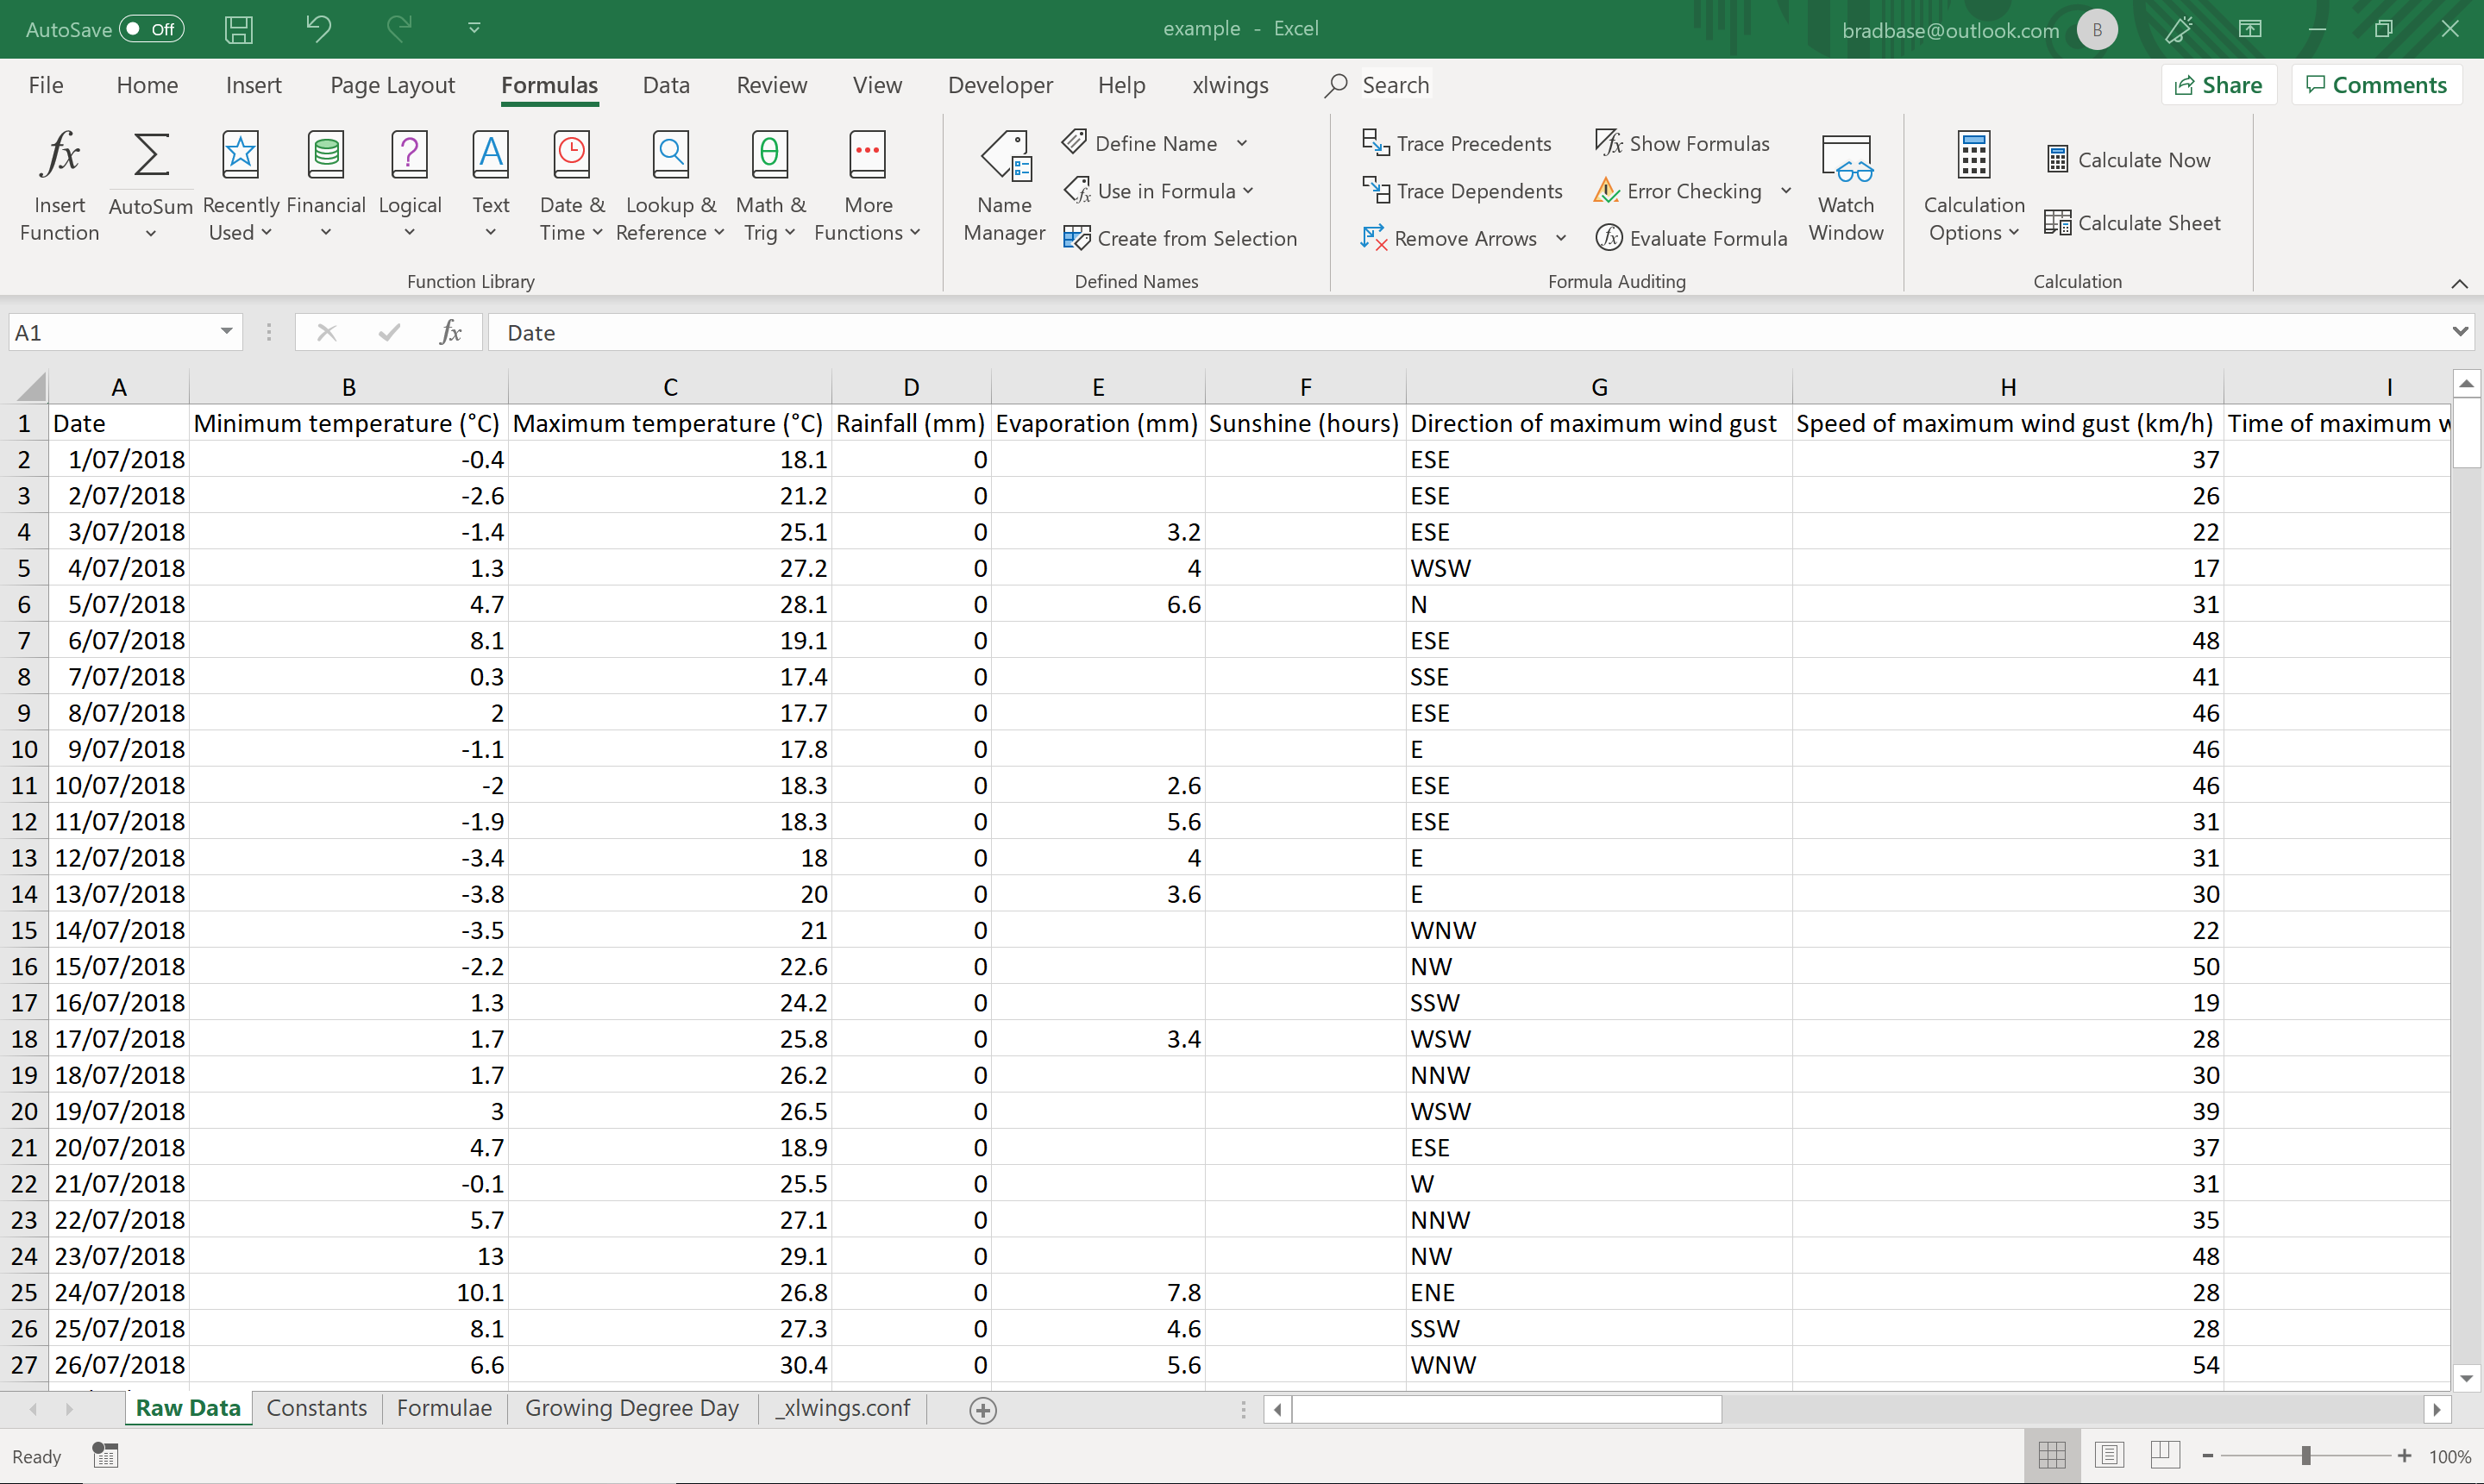
\includegraphics[scale=0.3]{images/raw_data.PNG}
	\caption{Raw Data}
\end{figure}

\paragraph{} After reading our \href{https://en.wikipedia.org/wiki/Growing_degree-day}{Growing Degree Day article on Wikipedia} we can see there is a term called $T_{\textrm{base}}$ (the base or reference temperature) and, according to the article, this value is usually defined as $10\degree\textrm{C}$ but this is open to change. So we will consider this a constant. \index{Constant}\index{$T_{\textrm{base}}$}

\begin{figure}[h!]
	\centering
	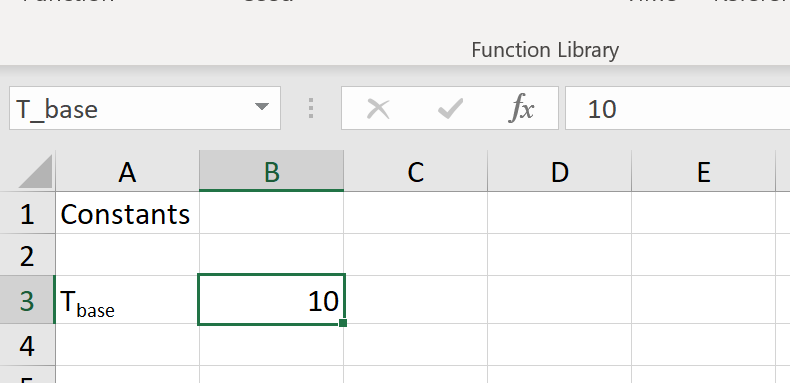
\includegraphics[scale=0.9]{images/t_base.PNG}
	\caption{$T_{\textrm{base}}$}
\end{figure}

\paragraph{} As can be seen in cell Constants!B3, we have the value 10. The cell Constants!B3 is a named range and it is called T\_base.\index{T\_base}

\paragraph{} Now for the Formulae tab. This is where the two formulas will be defined. The two formulae have a few variable terms in common, namely T\_min and T\_max. No prizes for figuring these are the daily minimum and maximum temperatures in degrees Celsius.\index{Formulae}

\paragraph{} The cell Formulae!C5 will be the the maximum temperature and Formulae!D5 will be the minimum. Again, both are named ranges.

\begin{itemize}
	\item Formulae!C5 is called T\_max \index{T\_min}
	\item Formulae!D5 is called T\_min \index{T\_max}
\end{itemize}

\begin{figure}[h!]
	\centering
	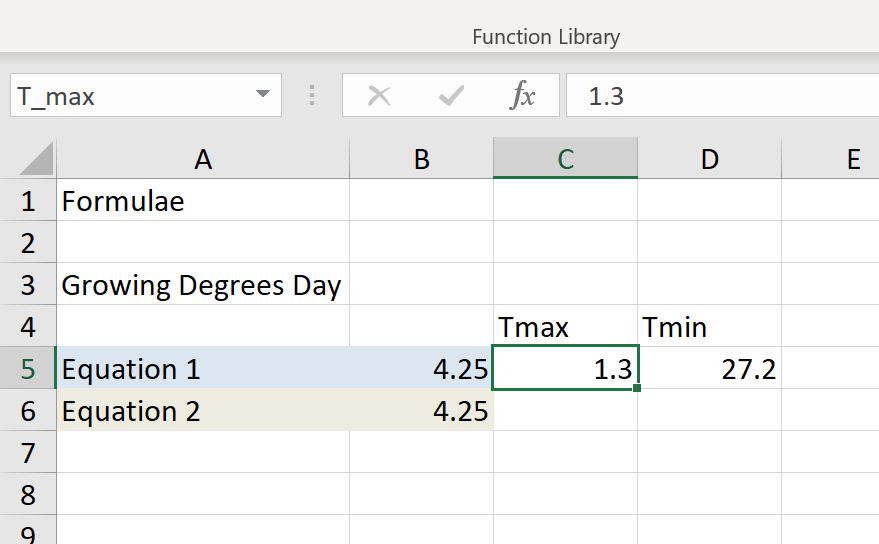
\includegraphics[scale=0.9]{images/t_max.PNG}
	\caption{$T_{\textrm{max}}$}
\end{figure}

\begin{figure}[h!]
	\centering
	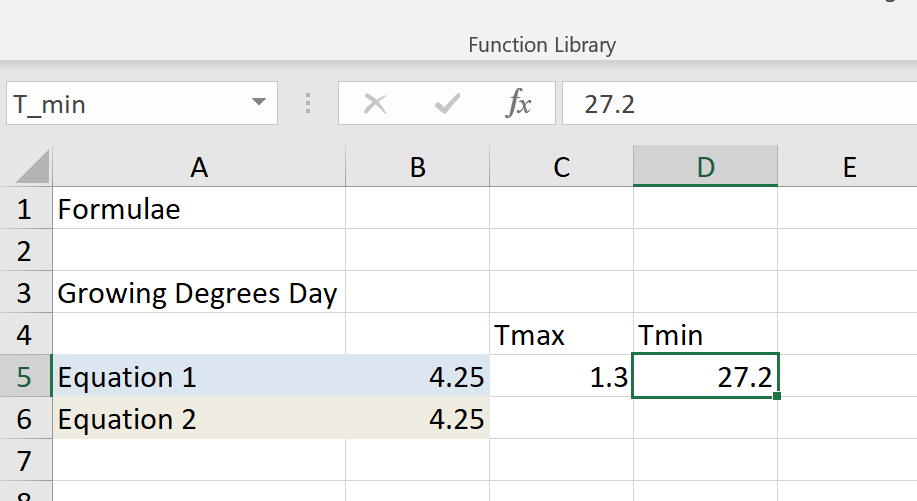
\includegraphics[scale=0.9]{images/t_min.PNG}
	\caption{$T_{\textrm{min}}$}
\end{figure}

\paragraph{} Label the variables (eg; something useful in Formulae!C4 and Formulae!D4).

\paragraph{} We will now define each of the Growing Degree Day models we want to explore. Be sure to use the named range of the variables and constants.\index{model}

\paragraph{} The use of named ranges and cell names is actually the ``secret'' behind making FlyingKoala work. By creating and using named ranges and cell names you are actually teaching Excel the language of your mathematical or technical model and Koala2 uses this acquired language to figure out how to run your calculations.

\paragraph{} Equation 1, from earlier, will be placed into Formulae!B5. In Excel's formula it looks like this:\index{Equation (1)}\index{Equation\_1}

$=$MAX( ((T\_max$+$T\_min)/2)$-$T\_base, 0 )

\paragraph{} Label the equation (eg; something useful in Formulae!A5)

\begin{figure}[h!]
	\centering
	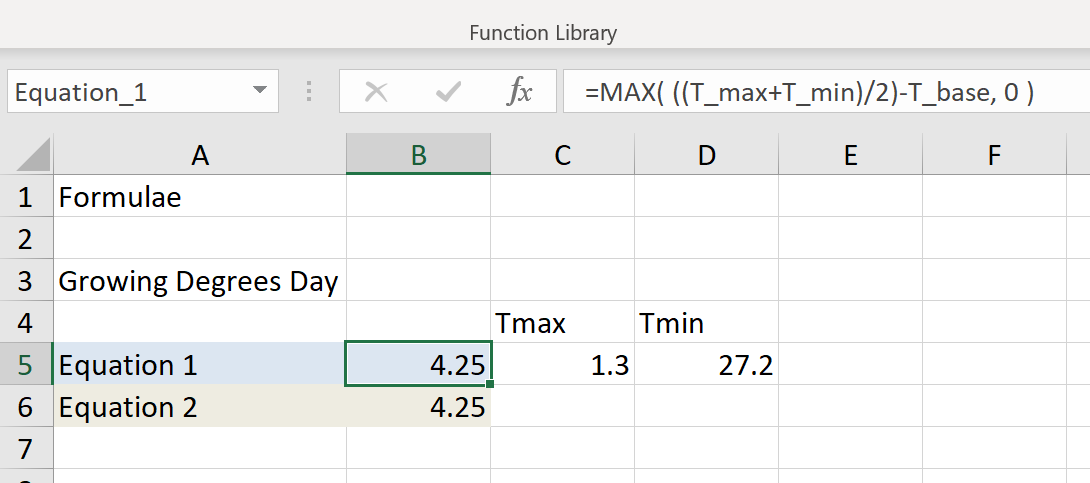
\includegraphics[scale=0.9]{images/equation_1.PNG}
	\caption{Equation (1)}
\end{figure}

\paragraph{} Equation 2, from earlier, will be placed into Formulae!B6. In Excel's formula it looks like this:\index{Equation (2)}\index{Equation\_2}

$=$IF(T\_min $<$ T\_base, ((T\_max$+$T\_base)/2)$-$T\_base, ((T\_max$+$T\_min)/2)$-$T\_base)

\paragraph{} Label the equation (eg; something useful in Formulae!A6)

\begin{figure}[h!]
	\centering
	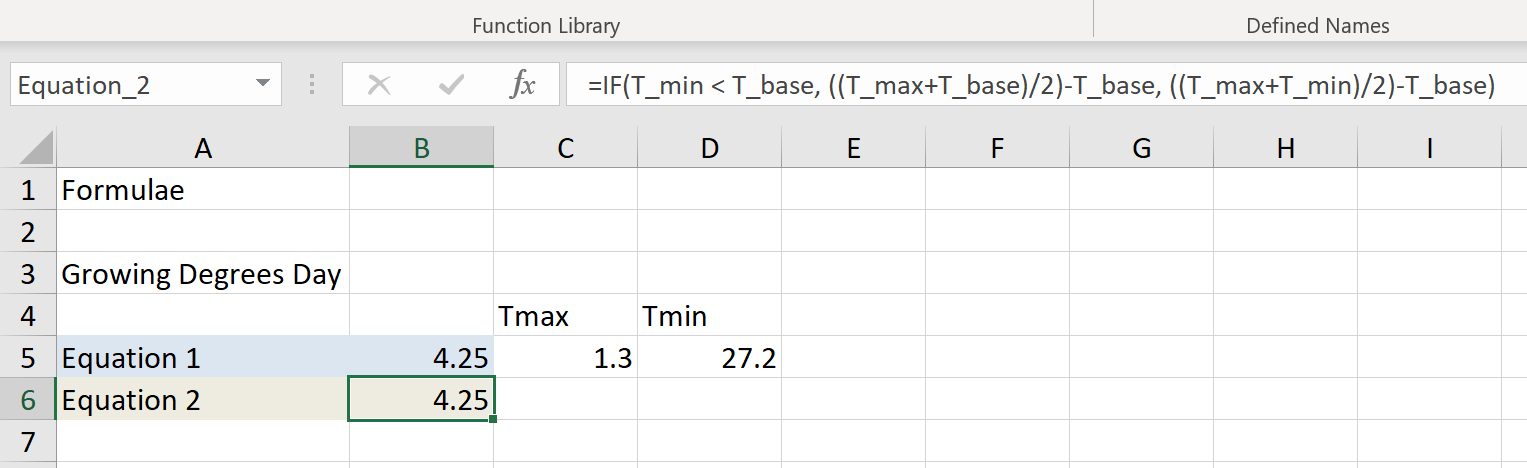
\includegraphics[scale=0.7]{images/equation_2.PNG}
	\caption{Equation (2)}
\end{figure}

\paragraph{} In both cases of Excel expressions for the equations we can see that;

\begin{itemize}
	\item Formulae!B5 is a named range called Equation\_1
	\item Formulae!B6 is a named range called Equation\_2
\end{itemize}


\subsection{Using your model(/s)}

\paragraph{} We will be using the worksheet Growing Degree Day. For this there is a need for some data and then we can use a User Defined Function to operate on the data.

\begin{itemize}
	\item ``Growing Degree Day''!A will be a label, in this case dates.
	\item ``Growing Degree Day''!B will be the minimum temperature.
	\item ``Growing Degree Day''!C will be the maximum temperature.
\end{itemize}

\paragraph{} ``Growing Degree Day''!D will a User Defined Function (UDF). This does require \textsl{some} code (but not much and is usually boilerplate / copy+paste). The code will be discussed later. The DegreeDay UDF is written in Excel as;\\

$=$DegreeDay(Equation\_1,\$B2,\$C2) \index{DegreeDay}

\begin{figure}[h!]
	\centering
	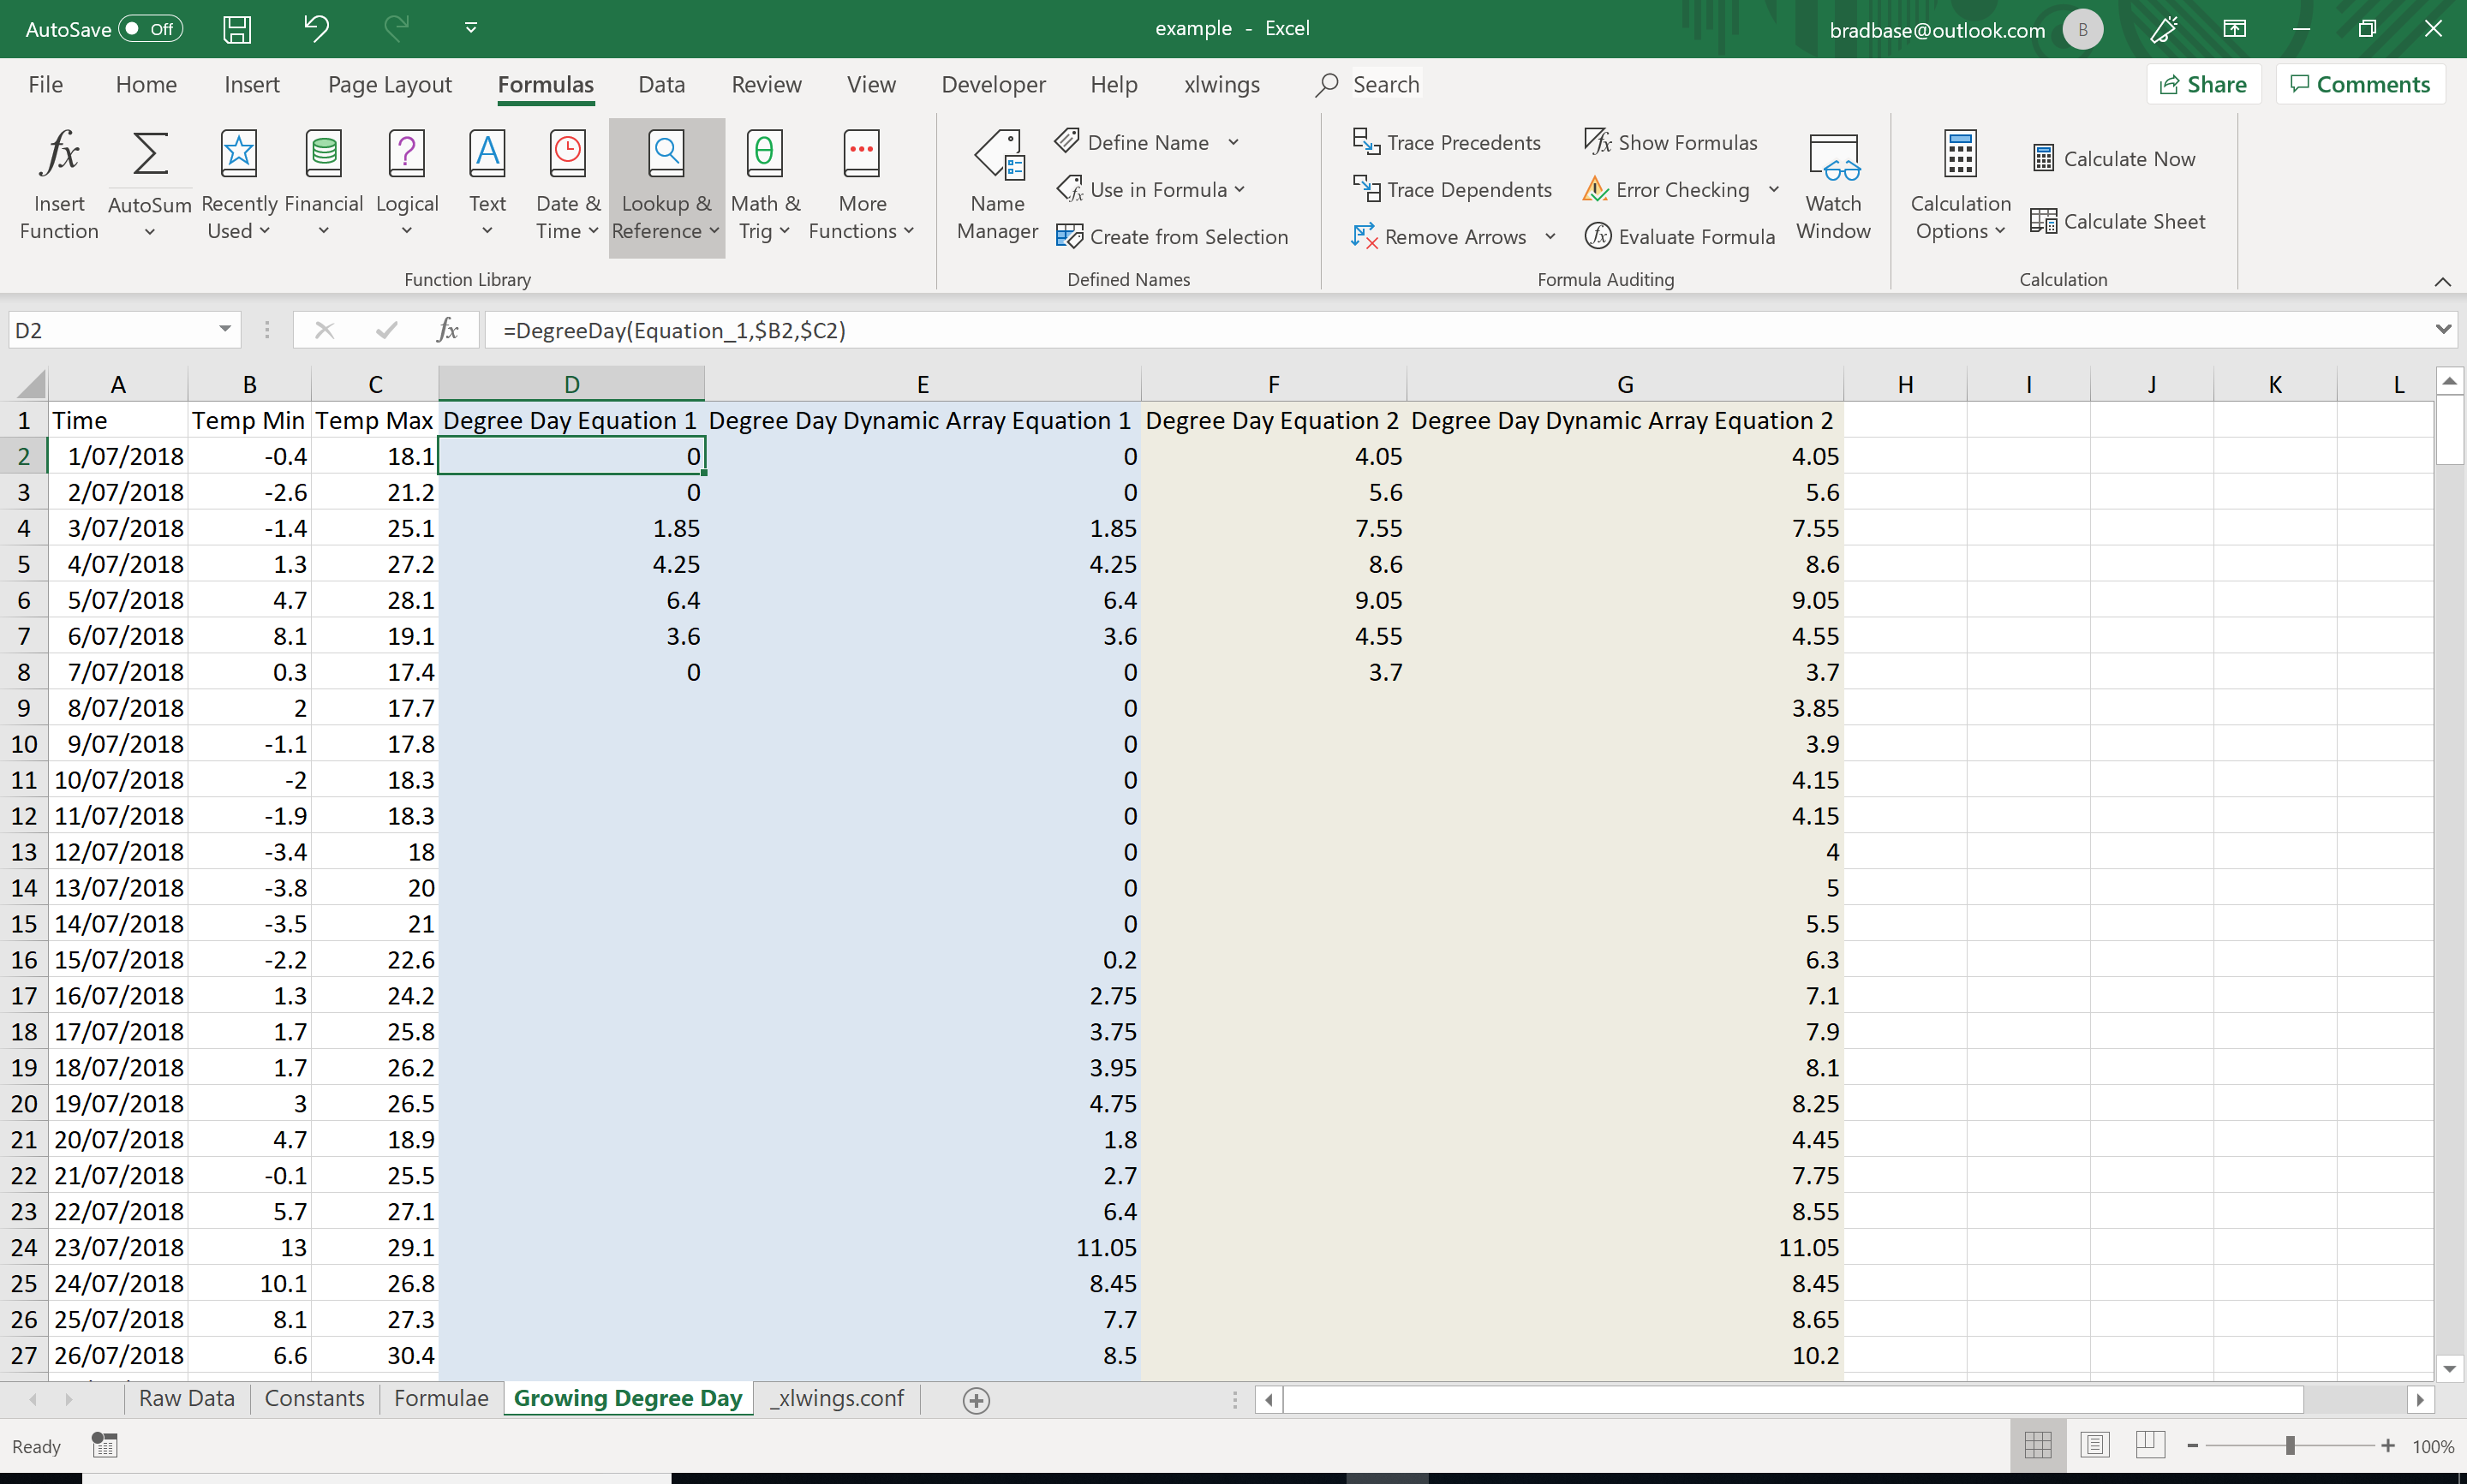
\includegraphics[scale=0.4]{images/degreeday_equation_1.PNG}
	\caption{Degree Day UDF Equation (1)}
\end{figure}

\paragraph{} Walking through the UDF called DegreeDay it presents as an integrated Excel formula. It even comes up as an option when you start typing. The code for DegreeDay function, however, is written in Python and executes in Python.

\paragraph{} The first argument for the DegreeDay function is the named range for the model we want to evaluate. In the above example this is Equation\_1.

\paragraph{} The second argument for the DegreeDay function is the minimum temperature. We can put a number in there but we are in Excel and would like to use the drag-down action so we will use a cell reference.

\paragraph{} The third argument for the DegreeDay function is the maximum temperature.  As with the minimum temperature we can put a number in there but we are in Excel and would like to use the drag-down action so we will use a cell reference.

\paragraph{} Like all functions in Excel, when you type it up right and hit enter, it'll evaluate and put the result in the cell you have defined it in. And you are welcome to do a fill-down to see it calculate for the entire series.

\paragraph{} Now for the leap...

\paragraph{} If you change the arguments on the DegreeDay UDF, you'll be using the second equation we had defined.\\

$=$DegreeDay(Equation\_2,\$B2,\$C2) \index{DegreeDay}

\paragraph{} Try it. Think about it. Enjoy it for a second.

\begin{figure}[h!]
	\centering
	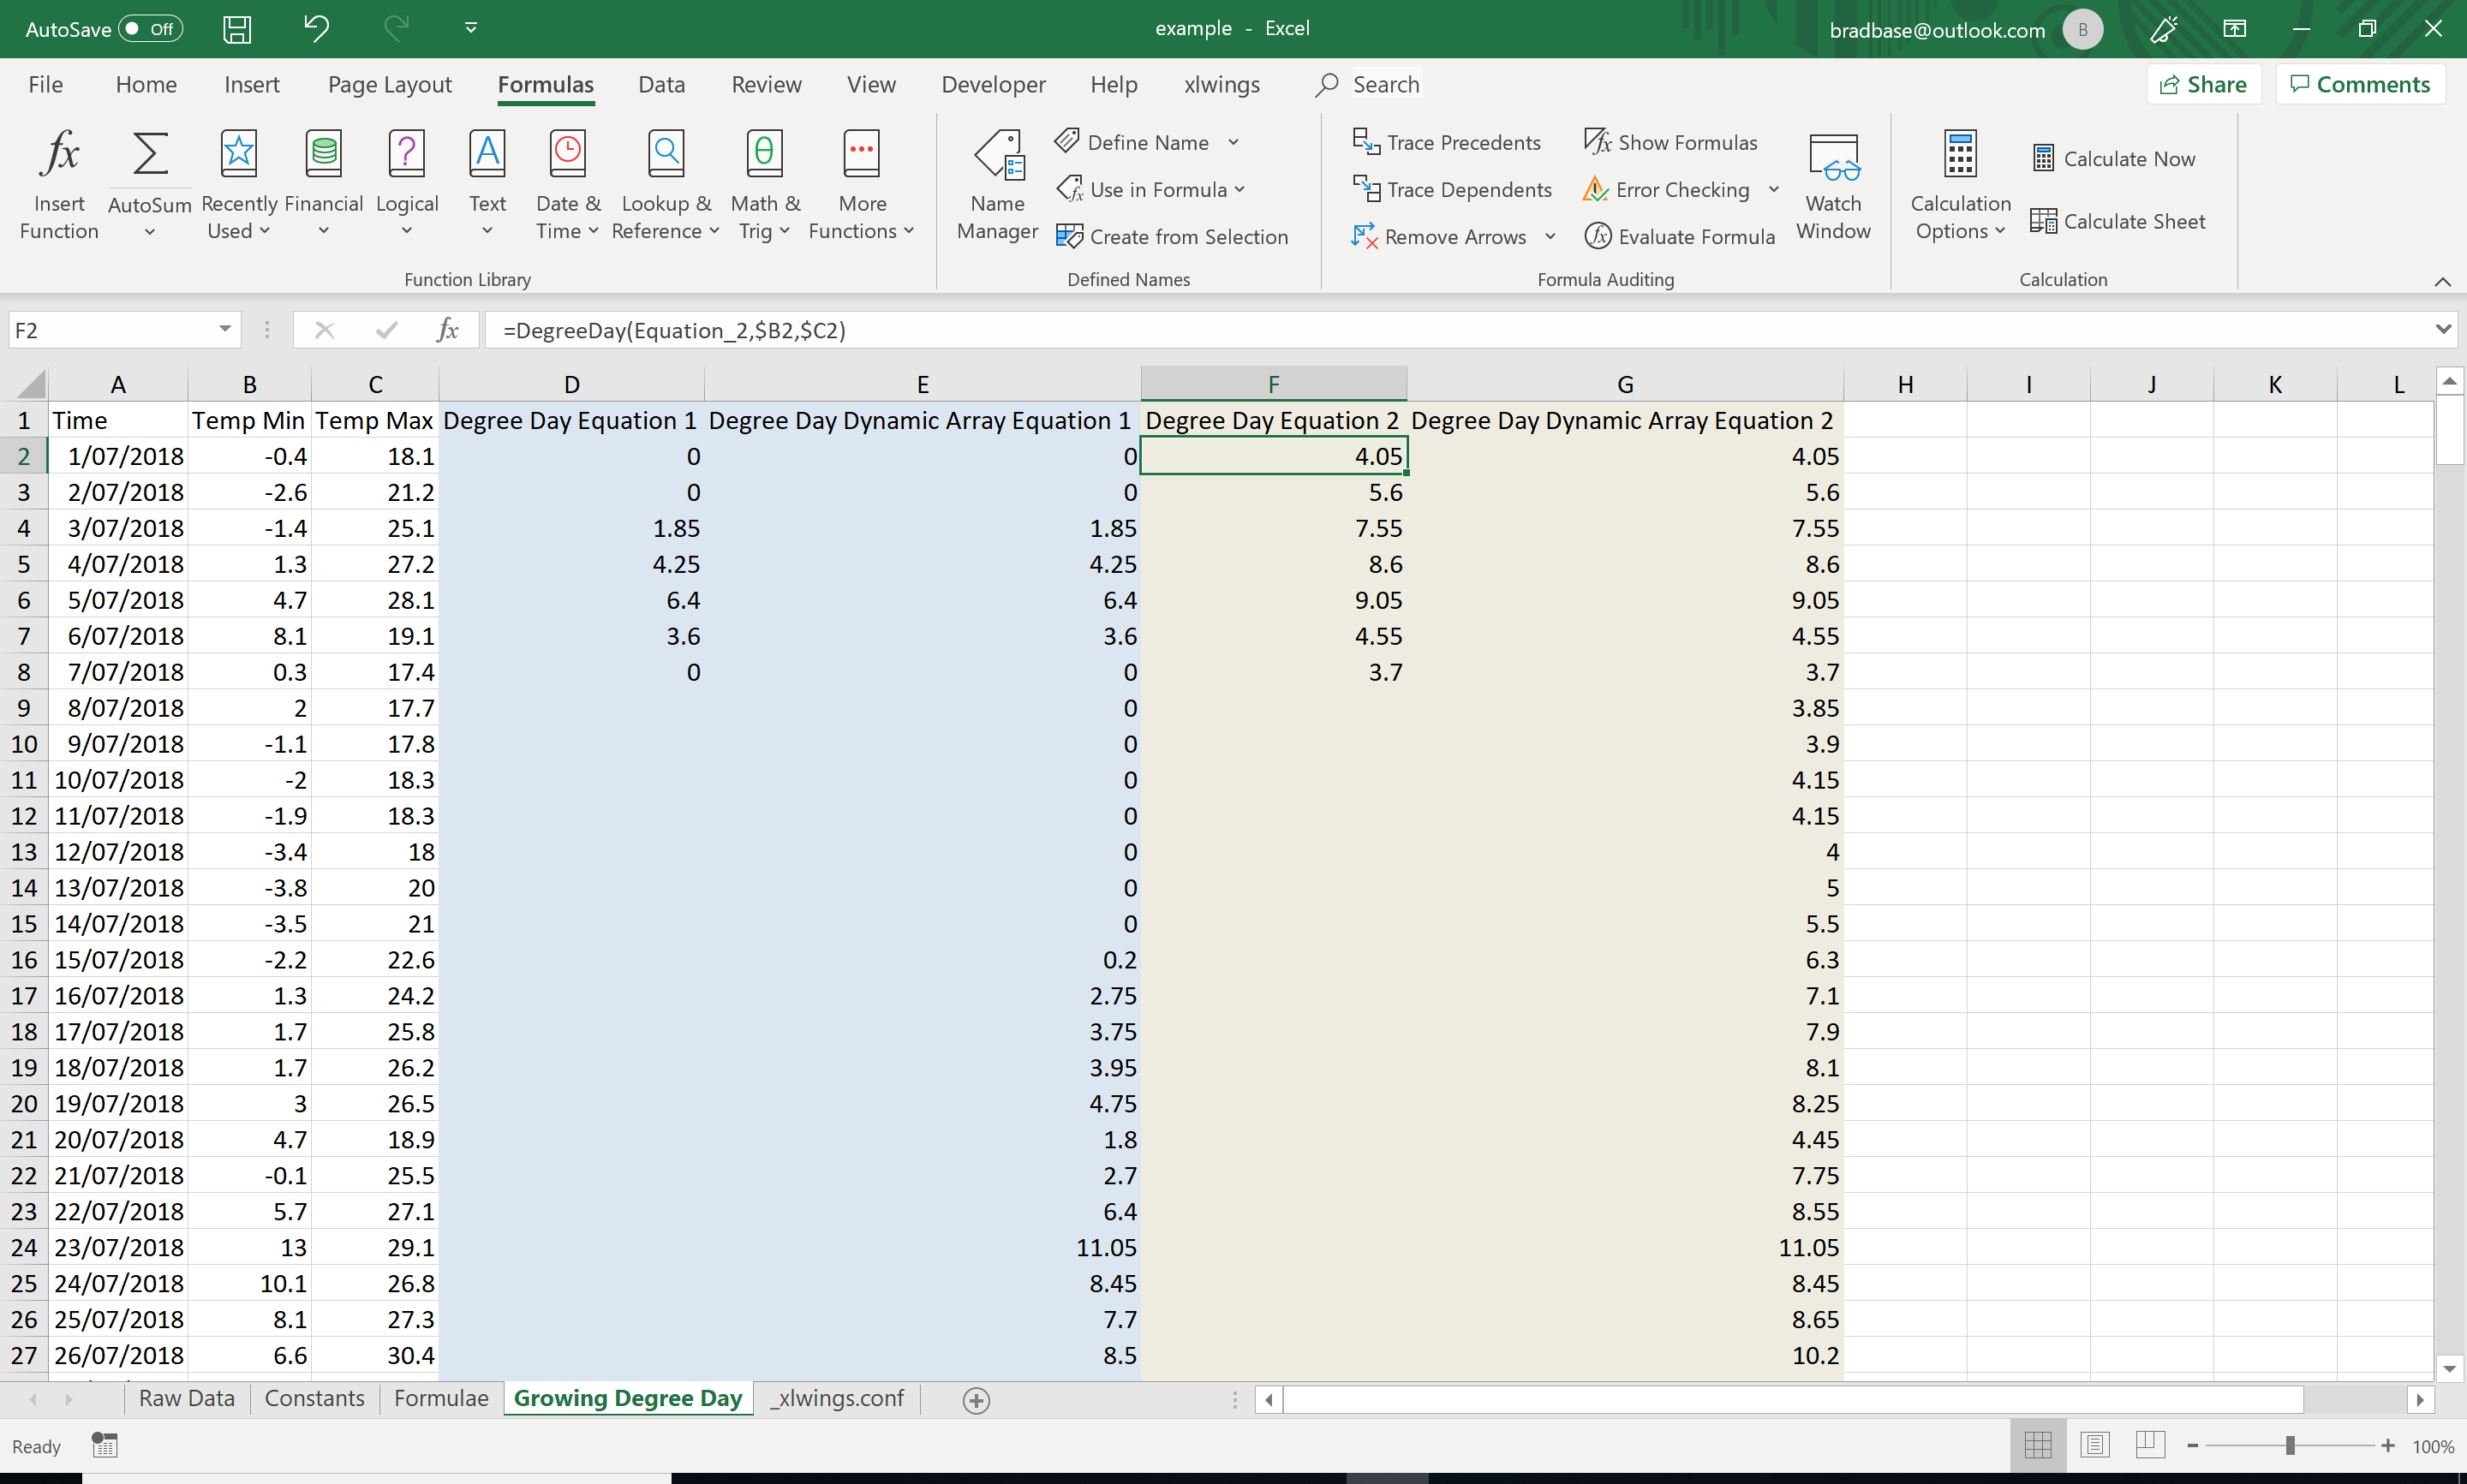
\includegraphics[scale=0.4]{images/degreeday_equation_2.PNG}
	\caption{Degree Day UDF Equation (2)}
\end{figure}

\paragraph{} This particular user defined function is great. We can see that FlyingKoala is using the same inputs on different equations and providing results. But, I'm certain you have already found, a fill-down for a years worth of data very quickly slows your computer down.

\paragraph{} Considering we may well be doing a lot of time series analysis we would not be able to live long enough for some calculations. Thankfully Excel provides a solution in the form of Dynamic Arrays. It's actually a solution that's been there a long time and can be used outside the context of FlyingKoala but very few people know how to take advantage of it. Thankfully, we can continue living in ignorance as FlyingKoala (actually, xlwings) has our back. We have available to us a second UDF which takes advantage of Dynamic Arrays. Creatively it's called DegreeDayDynamicArray.\\

$=$DegreeDayDynamicArray(Equation\_1,\$B2:\$B366,\$C2:\$C366) \index{DegreeDayDynamicArray}

\paragraph{} The only real usability difference between this function and the previous one is we can supply a range for the input of both the minimum and maximum temperatures. Providing the inputs are the same ``shape'' (they have the same number of rows), the result is an automatically filled in Dynamic Array with the results of the Equation\_1 for the series.

\begin{figure}[h!]
	\centering
	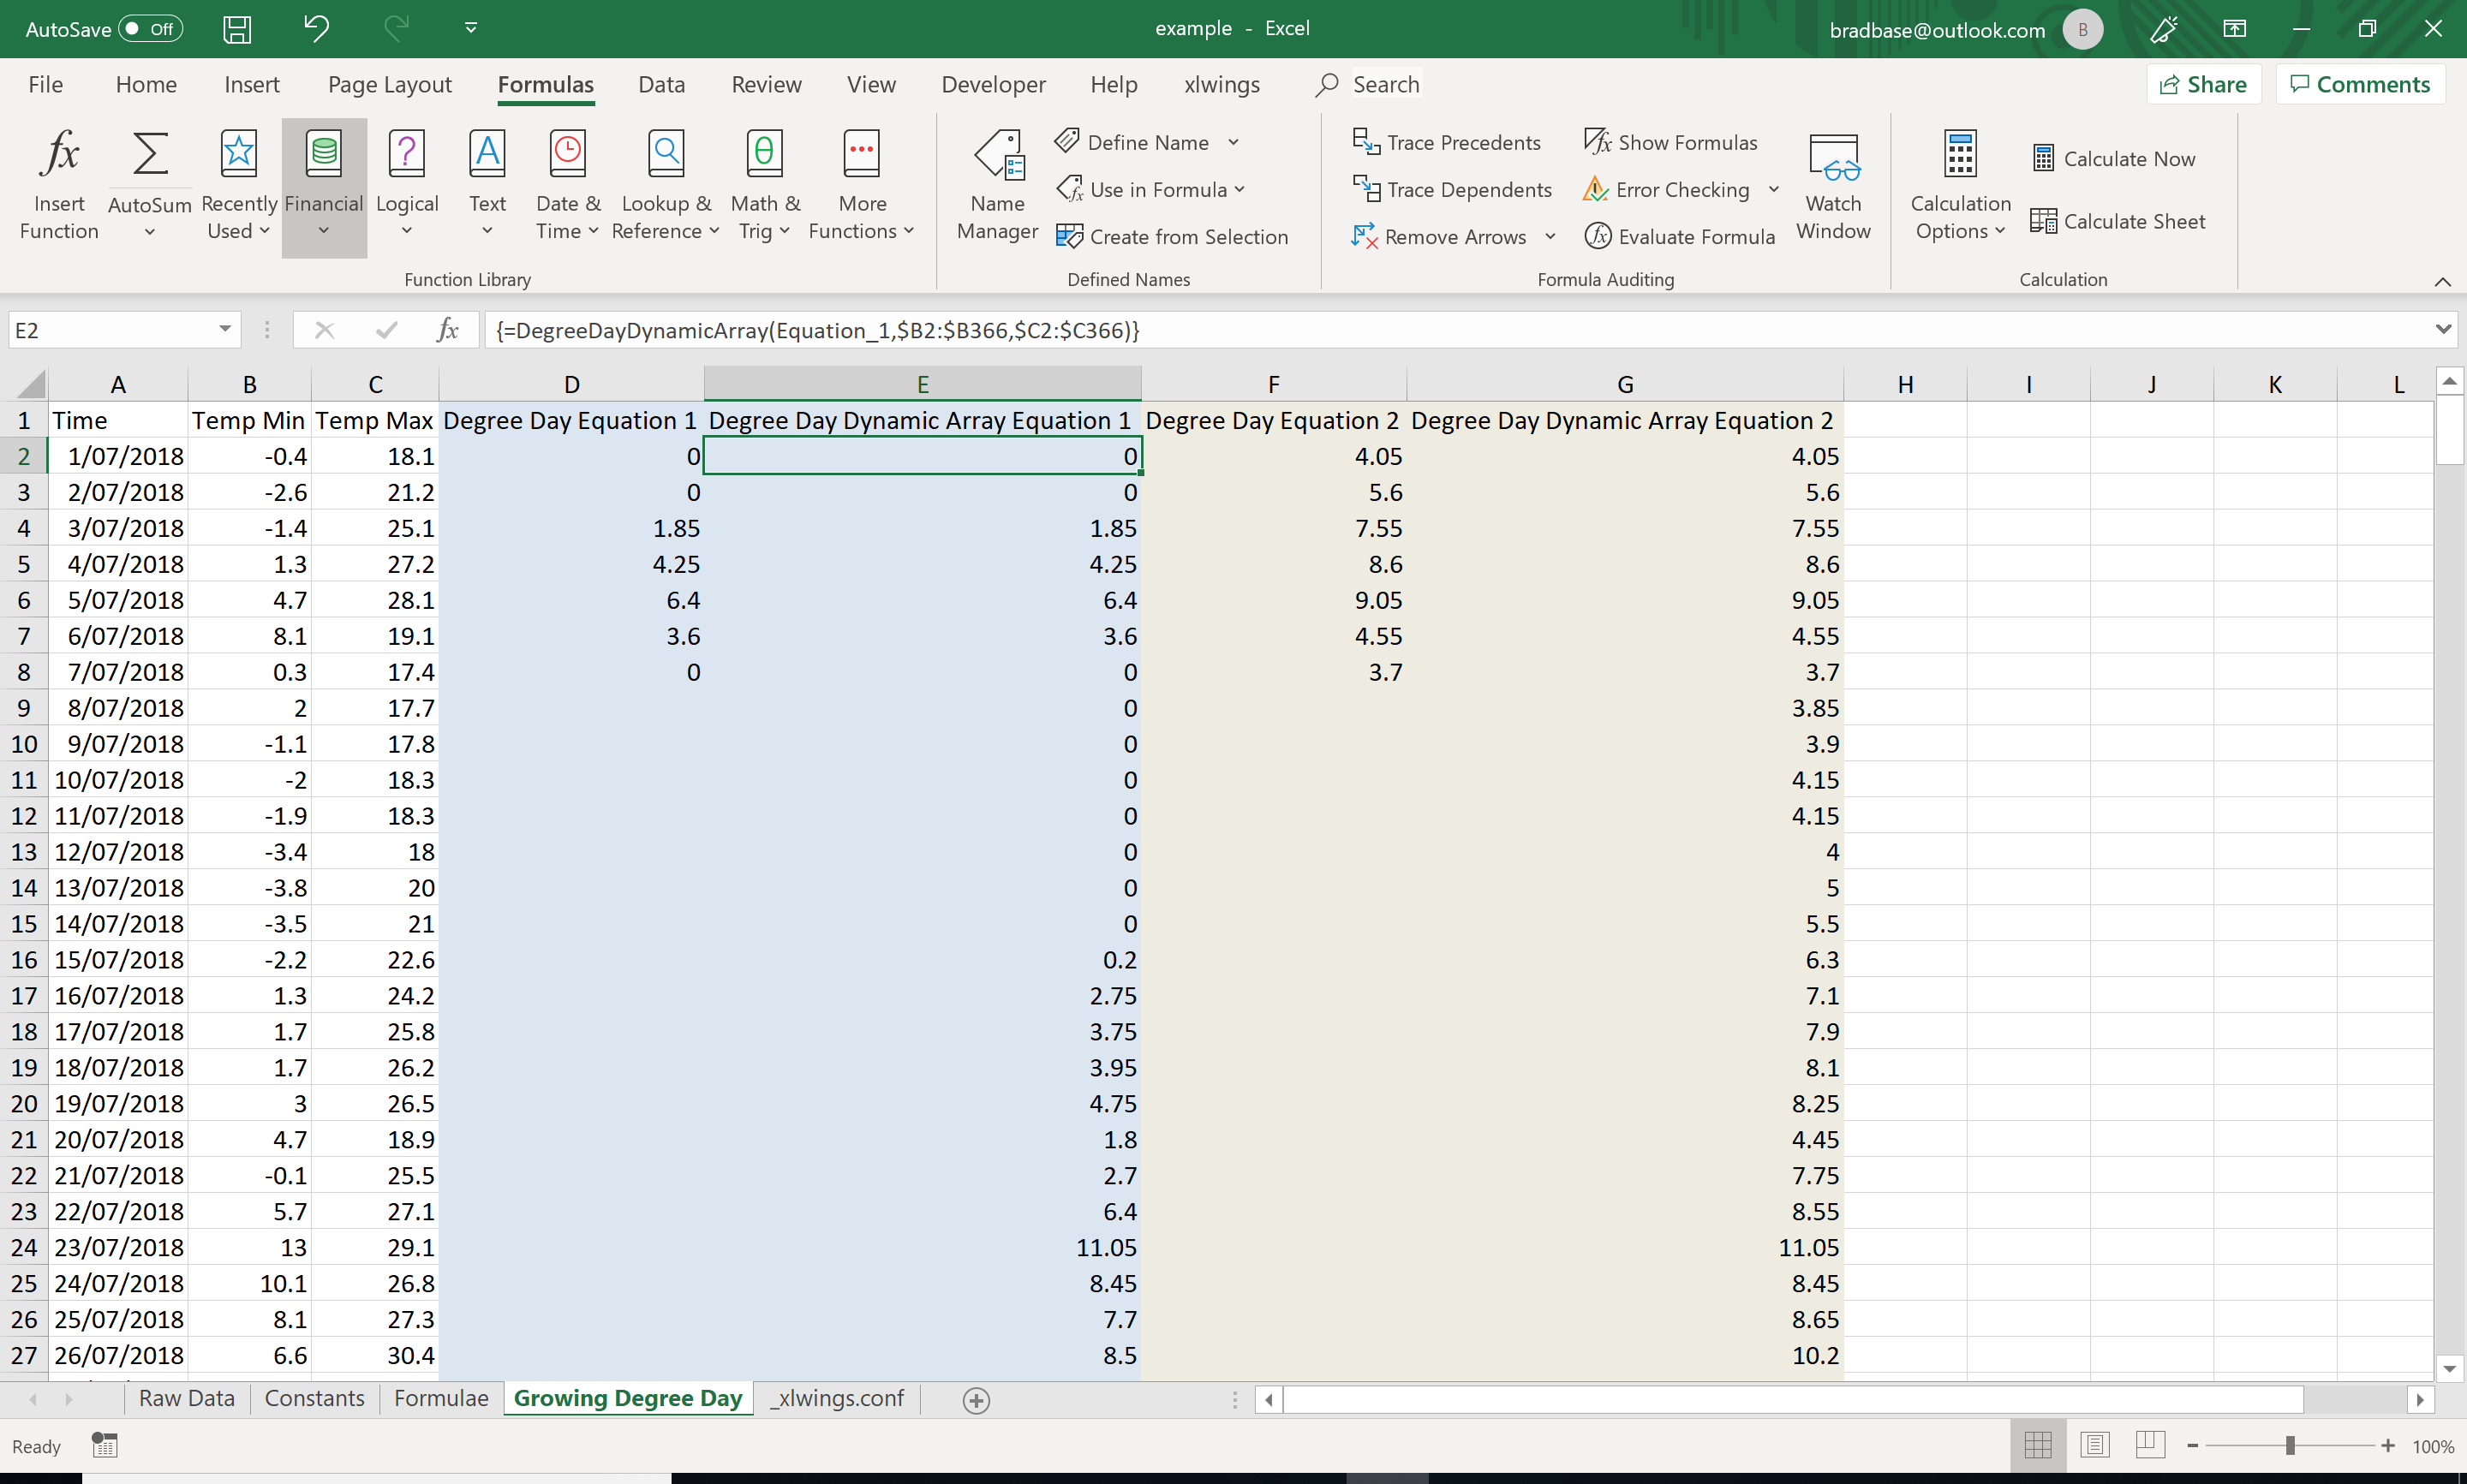
\includegraphics[scale=0.4]{images/degreedaydynamicarray_equation_1.PNG}
	\caption{Dynamic Array Equation (1)}
\end{figure}

\paragraph{} We can do the same for Equation\_2\\

$=$DegreeDayDynamicArray(Equation\_2,\$B2:\$B366,\$C2:\$C366) \index{DegreeDayDynamicArray}

\paragraph{} The Dynamic Array technique calculates results \textsl{really} quickly and can easily handle very big time series.

\begin{figure}[h!]
	\centering
	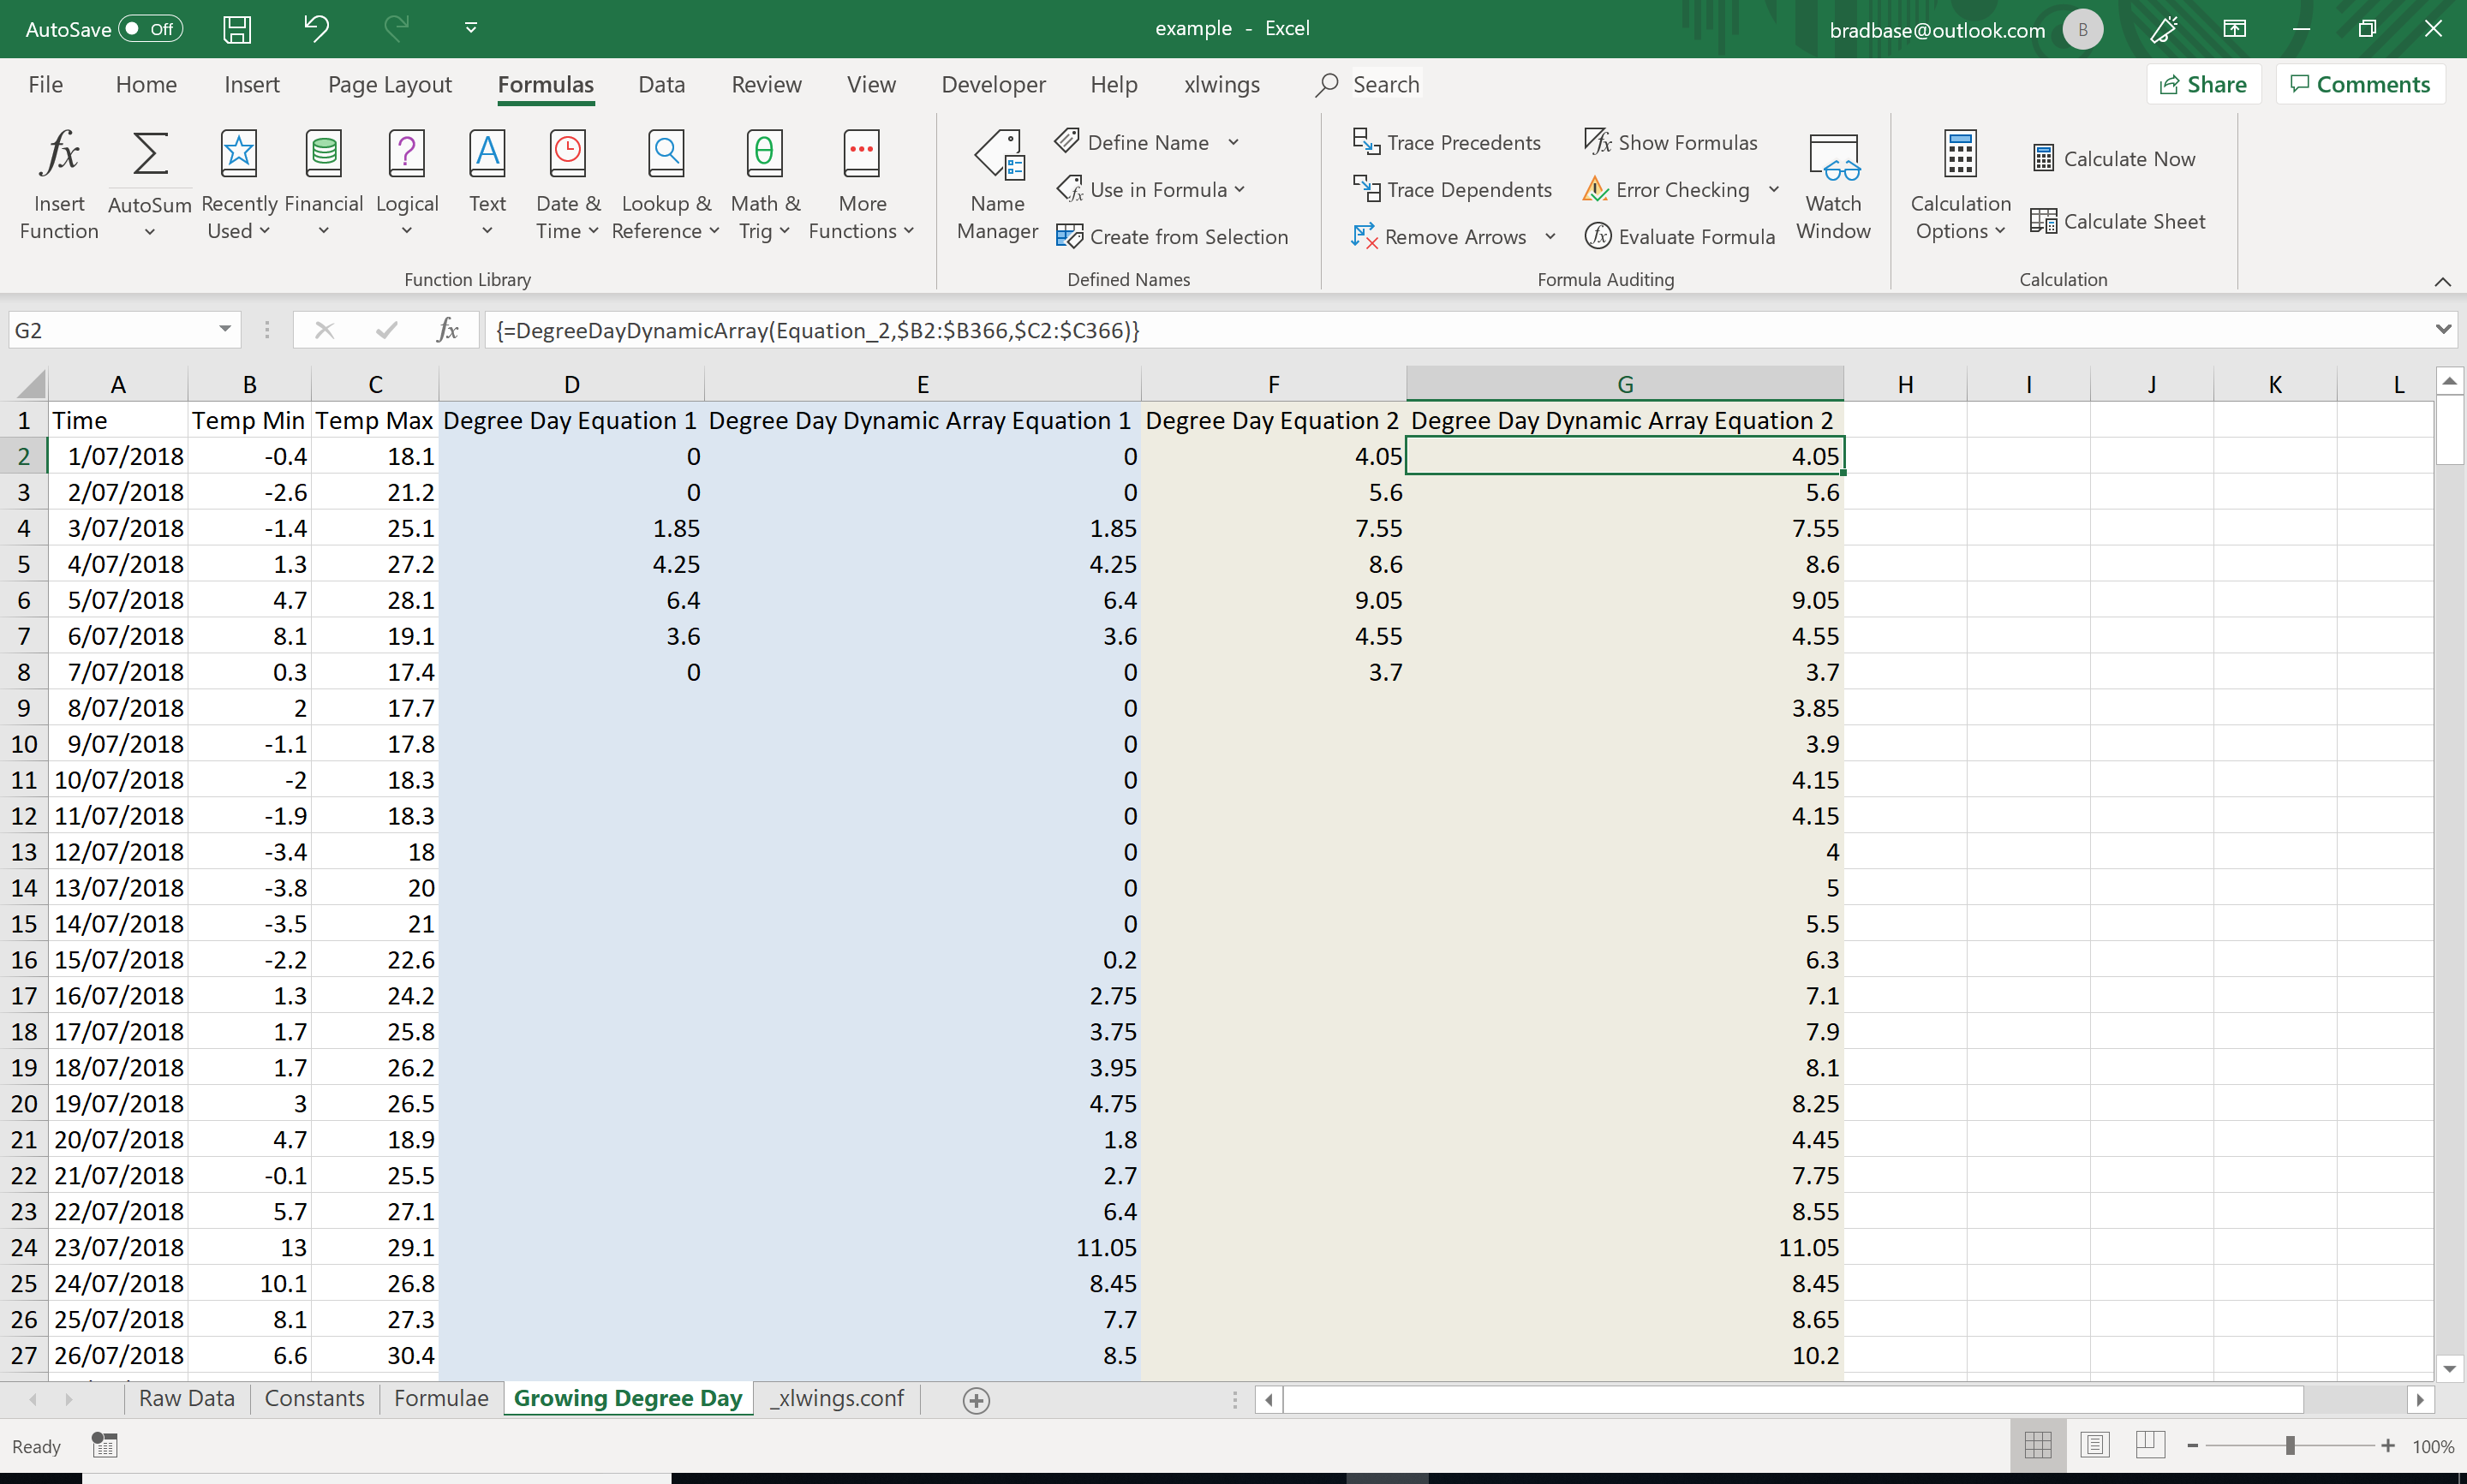
\includegraphics[scale=0.4]{images/degreedaydynamicarray_equation_2.PNG}
	\caption{Dynamic Array Equation (2)}
\end{figure}

\section{Under the hood (the code)}

\paragraph{} I have mentioned the code a couple of times. It is usually required to write a few UDFs as your domain is different from other people's. I am working on making FlyingKoala come with a collection of common ones but that's down the road a little and will require users to submit the ones they've written.

\paragraph{} From here I'll assume you know Python or are near someone who can fill you in on the gaps.

\paragraph{} This is the code you need to write to gain access to the pre-defined UDFs for DegreeDay and DegreeDayDynamicArray:

\begin{lstlisting}[language=Python]
import xlwings as xw
from flyingkoala import flyingkoala
from flyingkoala.horticulture import *
\end{lstlisting}

\paragraph{} Unless you have a need which falls outside the pre-defined UDFs, which will be defined in a document, the following sections are simply to illustrate how little code is required to support Excel equations defined by a domain expert.

\subsection{DegreeDay}

\paragraph{} The DegreeDay user defined function (UDF) is very literally a UDF as described by xlwings. If you are interested in writing UDFs I'll leave you to read from the xlwings doco. But we can see roughly 5 lines of code with a further 5 lines of mark-up.

\begin{lstlisting}[language=Python]
@xw.func
@xw.arg('model', xw.Range, doc='Name, as a string, of the model which will be evaluated. The Excel cell name / named range')
@xw.arg('T_min', np.array, doc='Daily minimum temperature')
@xw.arg('T_max', np.array, doc='Daily maximum temperature')
@xw.ret(index=False, header=False)
def DegreeDay(model, T_min, T_max):
    """Function to assemble a dataframe for calculating Degree Day"""

    if not isKoalaModelCached(model.name.name):
        generateModelGraph(model)

    inputs_for_DegreeDay = pd.DataFrame({'T_min': np.array([T_min]), 'T_max': np.array([T_max])})
    return EvaluateKoalaModel(model.name.name, inputs_for_DegreeDay)
\end{lstlisting}

\subsection{DegreeDayDynamicArray}

\paragraph{} Same goes for the DegreeDayDynamicArray UDF. As the terms T\_min and T\_max come in as numpy arrays we don't need to cast them.

\begin{lstlisting}[language=Python]
@xw.func
@xw.arg('model', xw.Range, doc='Name, as a string, of the model which will be evaluated. The Excel cell name / named range.')
@xw.arg('T_min', np.array, doc='Daily minimum temperature')
@xw.arg('T_max', np.array, doc='Daily maximum temperature')
@xw.ret(index=False, header=False, expand='down')
def DegreeDayDynamicArray(model, T_min, T_max):
    """Function to assemble a dataframe for calculating Degree Day using dynamic arrays"""

    if not isKoalaModelCached(model.name.name):
        generateModelGraph(model)

    inputs_for_DegreeDay = pd.DataFrame({'T_min': T_min, 'T_max': T_max})
    return EvaluateKoalaModel(model.name.name, inputs_for_DegreeDay)
\end{lstlisting}

\paragraph{} They key to a UDF is;
\begin{itemize}
	\item Unique name. You'll get bizarre errors if the UDF name is the same as a named range.
	\item model is always the first argument
	\item One parameter per term in your equation
\end{itemize}

\paragraph{} Obviously they can get more sophisticated. Calling out to databases, APIs, casting types, doing all sorts of other manipulations. It is Python so you've got everything here you'd want.

\newpage 
\printindex

\end{document}